 \def\bmode{2} % Mode 0 for presentation, mode 1 for a handout with notes, mode 2 for handout without notes
 \if 0\bmode
 \documentclass[smaller]{beamer}
 \else \if 1\bmode
 \immediate\write18{pdflatex -jobname=\jobname-Notes-Handout\space\jobname}
 \documentclass[smaller,handout]{beamer}
 \usepackage{handoutWithNotes}
 \pgfpagesuselayout{2 on 1 with notes}[letterpaper, landscape, border shrink=4mm]
 \else \if 2\bmode
 \immediate\write18{pdflatex -jobname=\jobname_Handout\space\jobname}
 \documentclass[smaller,handout]{beamer}
 \fi
 \fi
 \fi
% \documentclass[smaller, handout]{beamer}


% \documentclass[smaller,handout
% ]{beamer}
%\usepackage{etex}
%\newcommand{\num}{6{} }

% \usetheme[
%   outer/progressbar=foot,
%   outer/numbering=counter,
%  block=fillFF
% ]{metropolis}

%\useoutertheme{metropolis}

\usetheme{Madrid}
\useoutertheme[subsection=false]{miniframes} % Alternatively: miniframes, infolines, split
\useinnertheme{circles}
\usecolortheme{seahorse}

\usepackage[backend=biber,style=authoryear,maxcitenames=2,maxbibnames=99,safeinputenc,url=false,
eprint=false]{biblatex}
\addbibresource{bib/references.bib}
\AtEveryCitekey{\iffootnote{{\tiny}\tiny}{\tiny}}
\usepackage{appendixnumberbeamer}
%\usepackage{pgfpages}
%\setbeameroption{hide notes} % Only slides
%\setbeameroption{show only notes} % Only notes
%\setbeameroption{hide notes} % Only notes
%\setbeameroption{show notes on second screen=right} % Both

% \usepackage[sfdefault]{Fira Sans}

% \setsansfont[BoldFont={Fira Sans}]{Fira Sans Light}
% \setmonofont{Fira Mono}

%\usepackage{fira}
%\setsansfont{Fira}
%\setmonofont{Fira Mono}
% To give a presentation with the Skim reader (http://skim-app.sourceforge.net) on OSX so
% that you see the notes on your laptop and the slides on the projector, do the following:
% 
% 1. Generate just the presentation (hide notes) and save to slides.pdf
% 2. Generate onlt the notes (show only nodes) and save to notes.pdf
% 3. With Skim open both slides.pdf and notes.pdf
% 4. Click on slides.pdf to bring it to front.
% 5. In Skim, under "View -> Presentation Option -> Synhcronized Noted Document"
%    select notes.pdf.
% 6. Now as you move around in slides.pdf the notes.pdf file will follow you.
% 7. Arrange windows so that notes.pdf is in full screen mode on your laptop
%    and slides.pdf is in presentation mode on the projector.

% Give a slight yellow tint to the notes page
%\setbeamertemplate{note page}{\pagecolor{yellow!5}\insertnote}\usepackage{palatino}


%\usetheme{metropolis}
%\usecolortheme{beaver}
\usepackage{xcolor}
\definecolor{darkcandyapplered}{HTML}{A40000}
\definecolor{lightcandyapplered}{HTML}{e74c3c}

%\setbeamercolor{title}{fg=darkcandyapplered}
%\setbeamercolor{frametitle}{bg=darkcandyapplered!80!black!90!white}
%\setbeamertemplate{frametitle}{\bf\insertframetitle}
%\setbeamercolor{footnote mark}{fg=darkcandyapplered}
%\setbeamercolor{footnote}{fg=darkcandyapplered!70}
%\Raggedbottom
%\setbeamerfont{page number in head/foot}{size=\tiny}
%\usepackage[tracking]{microtype}


\setbeamertemplate{frametitle}{%
    \nointerlineskip%
    \begin{beamercolorbox}[wd=\paperwidth,ht=2.0ex,dp=0.6ex]{frametitle}
        \hspace*{1ex}\insertframetitle%
    \end{beamercolorbox}%
}



\setbeamerfont{caption}{size=\footnotesize}
\setbeamercolor{caption name}{fg=darkcandyapplered}


%\usepackage[sc,osf]{mathpazo}   % With old-style figures and real smallcaps.
%\linespread{1.025}              % Palatino leads a little more leading

% Euler for math and numbers
%\usepackage[euler-digits,small]{eulervm}
%\AtBeginDocument{\renewcommand{\hbar}{\hslash}}
\usepackage{graphicx,multirow,paralist,booktabs}


%\mode<presentation> { \setbeamercovered{transparent} }

\setbeamertemplate{navigation symbols}{}
\makeatletter
\def\beamerorig@set@color{%
  \pdfliteral{\current@color}%
  \aftergroup\reset@color
}
\def\beamerorig@reset@color{\pdfliteral{\current@color}}
\makeatother

%=== GRAPHICS PATH ===========
\graphicspath{{./images/}}
% Marginpar width
%Marginpar width
%\setlength{\marginparsep}{.02in}


%% Captions
% \usepackage{caption}
% \captionsetup{
%   labelsep=quad,
%   justification=raggedright,
%   labelfont=sc
% }

%AMS-TeX packages

\usepackage{amssymb,amsmath,amsthm} 
\usepackage{bm}
\usepackage{color}

\usepackage{hyperref,enumerate}
\usepackage{minitoc,array}


%https://tex.stackexchange.com/a/31370/2269
\usepackage{mathtools,cancel}

\renewcommand{\CancelColor}{\color{red}} %change cancel color to red

\makeatletter
\let\my@cancelto\cancelto %copy over the original cancelto command
\newcommand<>{\cancelto}[2]{\alt#3{\my@cancelto{#1}{#2}}{\mathrlap{#2}\phantom{\my@cancelto{#1}{#2}}}}
% redefine the cancelto command, using \phantom to assure that the
% result doesn't wiggle up and down with and without the arrow
\makeatother


\definecolor{slblue}{rgb}{0,.3,.62}
\hypersetup{
    colorlinks,%
    citecolor=blue,%
    filecolor=blue,%
    linkcolor=blue,
    urlcolor=slblue
}

%%% TIKZ
\usepackage{animate}
\usepackage{tikz}
\usepackage{pgfplots}
\usepackage{pgfplotstable}
\usepackage{pgfgantt}
\usepackage{tikzsymbols}
\pgfplotsset{compat=newest}
\usepgfplotslibrary{groupplots,fillbetween}

\usetikzlibrary{arrows,shapes,positioning,shapes.geometric}
\usetikzlibrary{decorations.markings}
\usetikzlibrary{shadows,automata}
\usetikzlibrary{patterns,matrix}
\usetikzlibrary{trees,mindmap,backgrounds}
%\usetikzlibrary{circuits.ee.IEC}
\usetikzlibrary{decorations.text}
% For Sagnac Picture
\usetikzlibrary{%
    decorations.pathreplacing,%
    decorations.pathmorphing%
}
\tikzset{no shadows/.style={general shadow/.style=}}
%
%\usepackage{paralist}



%%% FORMAT PYTHON CODE
%\usepackage{listings}
% Default fixed font does not support bold face
\DeclareFixedFont{\ttb}{T1}{txtt}{bx}{n}{8} % for bold
\DeclareFixedFont{\ttm}{T1}{txtt}{m}{n}{8}  % for normal

% Custom colors
\definecolor{deepblue}{rgb}{0,0,0.5}
\definecolor{deepred}{rgb}{0.6,0,0}
\definecolor{deepgreen}{rgb}{0,0.5,0}
 

%\usepackage{listings}

% Python style for highlighting
% \newcommand\pythonstyle{\lstset{
% language=Python,
% basicstyle=\footnotesize\ttm,
% otherkeywords={self},             % Add keywords here
% keywordstyle=\footnotesize\ttb\color{deepblue},
% emph={MyClass,__init__},          % Custom highlighting
% emphstyle=\footnotesize\ttb\color{deepred},    % Custom highlighting style
% stringstyle=\color{deepgreen},
% frame=tb,                         % Any extra options here
    % showstringspaces=false            %  Inference for Difference of Two Proportions
% }}

% % Python environment
% \lstnewenvironment{python}[1][]
% {
% \pythonstyle
% \lstset{#1}
% }
% {}

% % Python for external files
% \newcommand\pythonexternal[2][]{{
% \pythonstyle
% \lstinputlisting[#1]{#2}}}

% Python for inline
% 
% \newcommand\pythoninline[1]{{\pythonstyle\lstinline!#1!}}


\newcommand{\osn}{\oldstylenums}
\newcommand{\dg}{^{\circ}}
\newcommand{\lt}{\left}
\newcommand{\rt}{\right}
\newcommand{\pt}{\phantom}
\newcommand{\tf}{\therefore}
\newcommand{\?}{\stackrel{?}{=}}
\newcommand{\fr}{\frac}
\newcommand{\dfr}{\dfrac}
\newcommand{\ul}{\underline}
\newcommand{\tn}{\tabularnewline}
\newcommand{\nl}{\newline}
\newcommand\relph[1]{\mathrel{\phantom{#1}}}
\newcommand{\cm}{\checkmark}
\newcommand{\ol}{\overline}
\newcommand{\rd}{\color{red}}
\newcommand{\bl}{\color{blue}}
\newcommand{\pl}{\color{purple}}
\newcommand{\og}{\color{orange!90!black}}
\newcommand{\gr}{\color{green!40!black}}
\newcommand{\nin}{\noindent}
\newcommand{\la}{\lambda}
\renewcommand{\th}{\theta}
\newcommand{\al}{\alpha}
\newcommand{\G}{\Gamma}
\newcommand*\circled[1]{\tikz[baseline=(char.base)]{
            \node[shape=circle,draw,thick,inner sep=1pt] (char) {\small #1};}}

\newcommand{\bc}{\begin{compactenum}[\quad--]}
\newcommand{\ec}{\end{compactenum}}

\newcommand{\p}{\partial}
\newcommand{\pd}[2]{\frac{\partial{#1}}{\partial{#2}}}
\newcommand{\dpd}[2]{\dfrac{\partial{#1}}{\partial{#2}}}
\newcommand{\pdd}[2]{\frac{\partial^2{#1}}{\partial{#2}^2}}
\newcommand{\nmfr}[3]{\Phi\left(\frac{{#1} - {#2}}{#3}\right)}


\pgfmathdeclarefunction{poiss}{1}{%
  \pgfmathparse{(#1^x)*exp(-#1)/(x!)}%
  }

\pgfmathdeclarefunction{gauss}{2}{%
  \pgfmathparse{1/(#2*sqrt(2*pi))*exp(-((x-#1)^2)/(2*#2^2))}%
}

\pgfmathdeclarefunction{expo}{2}{%
  \pgfmathparse{#1*exp(-#1*#2)}%
}

\pgfmathdeclarefunction{expocdf}{2}{%
  \pgfmathparse{1 -exp(-#1*#2)}%
}

% \makeatletter
% \long\def\ifnodedefined#1#2#3{%
%     \@ifundefined{pgf@sh@ns@#1}{#3}{#2}%
% }

% \pgfplotsset{
%     discontinuous/.style={
%     scatter,
%     scatter/@pre marker code/.code={
%         \ifnodedefined{marker}{
%             \pgfpointdiff{\pgfpointanchor{marker}{center}}%
%              {\pgfpoint{0}{0}}%
%              \ifdim\pgf@y>0pt
%                 \tikzset{options/.style={mark=*, fill=white}}
%                 \draw [densely dashed] (marker-|0,0) -- (0,0);
%                 \draw plot [mark=*] coordinates {(marker-|0,0)};
%              \else
%                 \tikzset{options/.style={mark=none}}
%              \fi
%         }{
%             \tikzset{options/.style={mark=none}}        
%         }
%         \coordinate (marker) at (0,0);
%         \begin{scope}[options]
%     },
%     scatter/@post marker code/.code={\end{scope}}
%     }
% }

% \makeatother

\renewcommand{\arraystretch}{1.5}
%%%%%%%%%%%%%%%%%%%%%%%%%%%%%%%%%%%%%%%%%%%%%%%%%%%
%%%%%%%%%%%%%%%%%%%%%%%%%%%%%%%%%%%%%%%%%%%%%%%%%%%

\title[CEE 260/MIE 273 M6c: ANOVA]{{\normalsize CEE 260/MIE 273: Probability and Statistics in Civil Engineering} \\
Lecture M6c: Analysis of Variance (ANOVA)}
\date[\today]{\footnotesize \today}
\author{{\bf Jimi Oke}}
\institute[UMass Amherst]{
  \begin{tikzpicture}[baseline=(current bounding box.center)]
    \node[anchor=base] at (-7,0) (its) {\includegraphics[scale=.3]{UMassEngineering_vert}} ;
  \end{tikzpicture}
}

\newcommand{\hpp}{\hat{p_1} - \hat{p_2}}
\newcommand{\pp}{p_1 - p_2}    
\begin{document}

\maketitle




\begin{frame}
  \frametitle{Outline}
  \tableofcontents
\end{frame}

 





\section{Introduction}
\begin{frame}
	\frametitle{Inferences concerning two population variances}\pause
	It is sometimes necessary to compare two population variances (or standard deviations) using the sample sum of squares $S_1^2$ and $S_2^2$.\pause
	
	
	\bigskip
	
	\begin{minipage}{.45\linewidth}
		For this, the $F$-test is used. The test statistic is given by: \pause
		
		\pause
		
		\begin{equation}
			\label{eq:20}
			f = \fr{S_1^2/\sigma_1^2}{S_2^2/\sigma_2^2}
		\end{equation}
		\pause
		\begin{itemize}
			\item The $F$-distribution has 2 parameters: $\nu_1$ and $\nu_2$. \pause
			\item  Coined in 1934 by George W.\ Snedecor in honor of Sir Ronald A.\ Fisher \pause who developed the ANOVA method, among other achievements.
		\end{itemize}
	\end{minipage}\quad
	\begin{minipage}{.45\linewidth}
		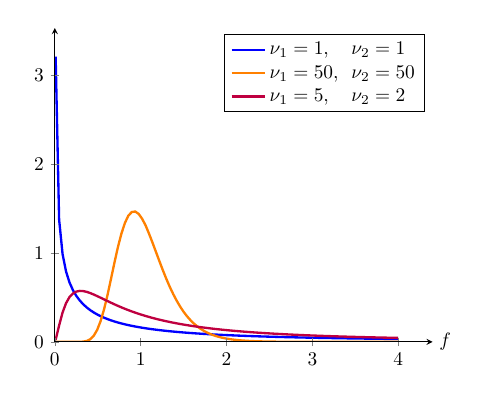
\begin{tikzpicture}[scale=.7,
			declare function={
				gamma(\z)=2.506628274631*sqrt(1/\z)+ 0.20888568*(1/\z)^(1.5)+ 0.00870357*(1/\z)^(2.5)- (174.2106599*(1/\z)^(3.5))/25920- (715.6423511*(1/\z)^(4.5))/1244160)*exp((-ln(1/\z)-1)*\z;
			},
			declare function={
				beta(\x,\y)=gamma(\x)*gamma(\y)/gamma(\x+\y);
			},
			declare function={
				fdst(\x,\a,\b) = 1 / beta(\a/2, \b/2) * (\a/\b)^(\a/2) * \x^(\a/2-1) * (1 + \a/\b*\x)^(-(\a + \b)/2);
			}
			]
			
			\begin{axis}[
				axis x line=center,
				xlabel=$f$,
				x label style={anchor=west},
				y label style={anchor=south},
				axis lines=left,
				axis on top,
				enlargelimits=upper,
				samples=100,
				xmin=0, ymin=0,
				domain=0.01:4,
				legend cell align=left
				]
				
				\addplot [very thick,blue] {fdst(x,1,1)}; \addlegendentry{$\nu_1=1,\hphantom{00} \nu_2=1$}
				\addplot [very thick,orange] {fdst(x,50,50)}; \addlegendentry{$\nu_1=50,\hphantom{0} \nu_2=50$}
				\addplot [very thick,purple] {fdst(x,5,2)}; \addlegendentry{$\nu_1=5,\hphantom{00} \nu_2=2$}
				
			\end{axis}
		\end{tikzpicture}    
	\end{minipage}
	
\end{frame}

\begin{frame}
	\frametitle{Analysis of Variance (ANOVA)}\pause
	So far, we have considered inference for:
	\begin{itemize}
		\item one-sample cases
		\item two-sample cases
	\end{itemize}
	\pause
	
	ANOVA is a methodology for comparing means across multiple groups. \\ \pause
	
	
	\begin{exampleblock}{Examples of experiments/studies requiring ANOVA} \pause
		\begin{itemize}
			\item Effects of five different brands of gasoline on automobile engine operating efficiency (mpg) \pause
			\item Effects of the presence of four different sugar solutions on bacterial growth \pause
			\item Investigating if hardwood concentration in pulp has an effect on tensile strength of bags made from the pulp \pause
			\item Deciding whether the color density of fabric specimens depends on the amount of dye used
		\end{itemize}
	\end{exampleblock}
	
\end{frame}

% \begin{frame}
	%   \frametitle{Key ANOVA definitions}\pause
	
	%   \begin{block}{Factor}\pause
		%     This is the differentiating quantity among populations  being studied
		%   \end{block}
	
	%   \pause
	
	%   \begin{block}{Level}
		%     Levels are the different treatments for a given factor. 
		%   \end{block}
	
	%   \pause
	
	% \end{frame}

\begin{frame}
	\frametitle{Single-factor ANOVA}
	\pause
	
	Comparison of more than two populations or treatment means. \\\pause
	
	\begin{eqnarray*}
		k &=& \text{number of populations/treatments} \\\pause
		\mu_1 &=& \text{mean of population 1 average response when treatment 1 is applied} \\\pause
		\vdots & \\ \pause
		\mu_k &=& \text{mean of population $k$ average response when treatment $k$ is applied} 
	\end{eqnarray*}
	
	\pause
	
	Hypotheses: \\\pause
	\begin{eqnarray*}
		H_0: & \mu_1 = \mu_2 = \cdots = \mu_k \\\pause
		H_1: & \text{at least two of the other $\mu_i$'s are different}
	\end{eqnarray*}
	
\end{frame}

\begin{frame}
	\frametitle{The ANOVA F-test}\pause
	
	\begin{description}
		\item[Assumption] All $k$ populations are normally distributed with means $\mu_i$ and equal variance $\sigma^2$. \pause{} The samples are independent and random.
		\item[Hypotheses]
		\begin{eqnarray*}
			H_0: & \mu_1 = \mu_2 = \cdots = \mu_k \\\pause
			H_1: & \text{at least one the other $\mu_i$'s differs from the others}
		\end{eqnarray*}
		\item[Test Statistic]
		\begin{equation*}
			f = \fr{\text{mean square among groups}}{\text{mean square error}}
		\end{equation*}
		\item[Compare]
		\begin{enumerate}[(a)]
			\item Find critical value $F_{1-\alpha, \nu_1,\nu_2}$.\\ \pause
			If $f \le F_{1-\alpha, \nu_1,\nu_2}$, \textbf{fail to reject $\bm{H_0}$}  \pause \textit{OR} \\\pause
			\item Find $p$-value. \\ \pause
			If $\alpha \le  p$-value, \textbf{fail to reject $\bm{H_0}$}
		\end{enumerate}
	\end{description}
\end{frame}



\section{One-way ANOVA}

% \begin{frame}
	%   \frametitle{Single-factor (one-way) ANOVA}
	%   \pause
	
	%   Comparison of more than two populations or treatment means. \\\pause
	
	%   \begin{eqnarray*}
		%     k &=& \text{number of populations/treatments} \\\pause
		%     \mu_1 &=& \text{mean of population 1/true average response when treatment 1 is applied} \\\pause
		%     \vdots & \\ \pause
		%     \mu_k &=& \text{mean of population k/true average response when treatment k is applied} 
		%   \end{eqnarray*}
	
	%   \pause
	
	%   Hypotheses: \\\pause
	%   \begin{eqnarray*}
		%     H_0: & \mu_1 = \mu_2 = \cdots = \mu_k \\\pause
		%     H_1: & \text{at least two of the other $\mu_i$'s are different}
		%   \end{eqnarray*}
	
	% \end{frame}

% % \begin{frame}
	% %   \frametitle{}
	% % \end{frame}

% \begin{frame}
	%   \frametitle{Assumptions}
	
	%   Key assumptions of ANOVA:
	
	%   \begin{itemize}
		%   \item Each treatment population (or group) is normally distributed with the same variance $\sigma^2$
		%   \item The samples for each level are independent
		%   \end{itemize}
	% \end{frame}

\begin{frame}
	\frametitle{Different sums of squares in ANOVA}\pause
	
	\begin{block}{Total sum of squares ($SST$)}
		\begin{equation}
			\label{eq:sst}
			SST = \sum_{i=1}^k \sum_{j=1}^{n_i} (x_{ij} - \ol{x})^2 
		\end{equation}
		where: \pause
		\begin{itemize}
			\item $x_{ij}$ is the observed quantity $j$ in group $i$ \pause
			\item $n_i$ is the number of observations (sample size) in group $i$ \pause
			\item $\ol{x}$ is the \textbf{grand mean} from all $k$ samples: \pause
			\begin{equation}
			\ol{x} = \fr 1n	\sum_{i=1}^k \sum_{j=1}^{n_i} x_{ij}
			\end{equation} 
			\pause and $n = n_1 + n_2 + \cdots + n_k$
		\end{itemize}

	\end{block}
	
	
\end{frame}

\begin{frame}
	\frametitle{Different sums of squares in ANOVA (cont.)}\pause
	
	\begin{block}{Sum of squares between groups ($SSG$)}\pause
				Measures the variance \textit{among} the $k$ sample means	
		
		\begin{equation}
			\label{eq:ssg}
			SSG = \sum_{i=1}^k n_i(\ol{x_i} - \ol{x})^2
		\end{equation}
\pause
(Also called \textbf{sum of squares for treatments} ($SSTr$))
	\end{block}
	\pause
	\begin{block}{Sum of squares for error ($SSE$)}\pause
				Measures the pooled variance \textit{within} each of the $k$ samples\pause
		\begin{equation}
			\label{eq:sse}
			SSE = (n_1 - 1)s_1^2 + (n_2 - 1)s_2^2 + \cdots + (n_k - 1)s_k^2 = \sum_{i=1}^k (n_i - 1)s_i^2
		\end{equation}\pause
	where $s_i^2$ is the sample variance for group $i$. 
	\end{block}
\end{frame}

\begin{frame}
	\frametitle{Fundamental identities and d.o.f.}
	
	\pause
	
	\begin{block}{Fundamental identity}\pause
		\begin{equation}
			\label{eq:funi}
			SST = SSG + SSE
		\end{equation}
		(You can prove this identity as an exercise.)
	\end{block}
	
	\pause
	
	Degrees of freedom (df): \\ \pause
	
	\begin{eqnarray}
		df(SST) &=& n - 1 \\ \pause
		df(SSG)  &=& k - 1 \\ \pause
		df(SSE)  &=& n - k 
	\end{eqnarray}
	\pause
		It also follows that:
	
	\begin{equation}
		\label{eq:dfi}
		df(SST) =  df(SSG) +   df(SSE)
	\end{equation}
\end{frame}


\begin{frame}
	\frametitle{Variances among and within groups}
	Ultimately, we want to determine how the variance is porportioned among the samples.\\ \pause
	
	\bigskip
	
	%Recall that the variance estimator is given by the sum of squared deviations divided by the d.o.f. Thus, we have the following variance estimates: \pause
	
	\begin{block}{Mean square among groups (MSG)}
		\begin{equation}
			\label{eq:msg}
			MSG \pause = \fr{1}{k-1}\times SSG  \pause = \fr{1}{k-1}\sum n_i(\ol{x_i} - \ol{x})^2
		\end{equation}
		
		\begin{itemize}
			\item Variance among the groups/treatments
			\item Also called \textbf{mean square for treatments} (MSTr)
		\end{itemize}
		
	\end{block}
	
	\pause
	
	\begin{block}{Mean square [for] error (MSE)}
		\begin{equation}
			\label{eq:msg}
			MSE \pause = \fr{1}{n-k}\times SSE \pause = \fr{1}{n-k} \sum_{i=1}^k (n_i - 1)s_i^2
		\end{equation}
		
		\pause
		\begin{itemize}
			\item Pooled variance within each of the groups.
		\end{itemize}
	\end{block}
\end{frame}


\begin{frame}
	\frametitle{Summary of ANOVA notation and sums}\pause
	\vspace{-5ex}
	\begin{eqnarray*}
		k &=& \text{number of groups/samples/treatments/populations} \\\pause
		n &=& n_1 + n_2 + \cdots + n_k \\\pause
		\ol{x} &=& \fr1n\sum x_{ij} \quad \text{(grand mean)} \\\pause
		SST &=& \sum (x_{ij} - \ol{x})^2  = \sum x_{ij}^2 - CM \\\pause
		SSG &=& \sum_{i=1}^k n_i(\ol{x_i} - \ol{x})^2 = \sum\fr{T_i^2}{n_i} - CM \\\pause
		T_i &=& \sum_j x_{ij} \quad \text{(total of the observations for group $i$)} \\
		CM &=& \fr1n\lt(\sum x_{ij}\rt)^2 \quad \text{(correction for the mean)} \\	\pause	
		SSE &=&  \sum_{i=1}^k (n_i - 1)s_i^2 = SST - SSG \\\pause
		MSG &=& \fr{1}{k-1}SSG \qquad  MSE = \fr{1}{n-k}SSE
	\end{eqnarray*}
\end{frame}

\begin{frame}
	\frametitle{Test statistic}\pause
	
	The test procedure compares a {\rd measure of differences among the sample means (``between-samples'' variation)}\pause{} to a \pause{}
	{\bl measure of variation calculated from within each of the samples.}
	
	\begin{block}{Test statistic for one-way ANOVA}\pause
		\begin{equation}
			\label{eq:20}
			F = \fr{\rd MSG}{\bl MSE}
		\end{equation}
		\pause
		\begin{itemize}
			\item $H_0: \mu_1 = \mu_2 = \cdots = \mu_k$ \pause
			\item $\bl MSE$ is an unbiased estimate of $\sigma^2$ whether or not $H_0$ is true  \pause
			\item $\rd MSG$ is an unbiased estimate of $\sigma^2$ ONLY when $H_0$ is true \pause 
			\item When $H_0$ is not true, $\mathbb{E}({\rd MSG}) > \mathbb{E}({\bl MSE}) = \sigma^2 \implies f > 1$ \pause
			\item When $H_0$ is true, $f$ follows the $F$-distribution with: \pause 
			\begin{eqnarray}
				 \nu_1 &=& k-1 \\ \pause 
				 \nu_2 &=& n-k
			\end{eqnarray}
		\end{itemize}
	\end{block}
\end{frame}

\begin{frame}
	\frametitle{The ANOVA F-test}\pause
	
	\begin{description}
		\item[Assumption] All $k$ populations are normally distributed with means $\mu_i$ and equal variance $\sigma^2$. \pause{} The samples are independent and random.
		\item[Hypotheses]
		\begin{eqnarray*}
			H_0: & \mu_1 = \mu_2 = \cdots = \mu_k \\\pause
			H_1: & \text{at least one the other $\mu_i$'s differs from the others}
		\end{eqnarray*}
		\item[Test Statistic]
		\begin{equation*}
			f = \fr{MSG}{MSE}
		\end{equation*}
		\item[Compare]
		\begin{enumerate}[(a)]
			\item Find critical value $F_{1-\alpha, \nu_1,\nu_2}$\footnote{Use \texttt{\rd finv(1 - alpha, nu1, nu2)} in MATLAB} (also called $f^*$).\\ \pause
			If $f \le F_{1-\alpha, \nu_1,\nu_2}$, \textbf{fail to reject $\bm{H_0}$}  \pause \textit{OR} \\\pause
			\item Find $p$-value. \\ \pause
			If $\alpha \le  p$-value, \textbf{fail to reject $\bm{H_0}$}
		\end{enumerate}
	\end{description}
\end{frame}


\section{ANOVA table}
\begin{frame}
	\frametitle{ANOVA table}
	When conducting one-way ANOVA, computations are usually summarized in an ANOVA table\pause
	
	\begin{table}
		\centering
		\begin{tabular}{l l l l c} \toprule 
			\bf Source of & \bf d.o.f. & \bf Sum of  & \bf Mean Square & $\bm f$ \\
			\bf  variation &       & \bf Squares & & \\ \midrule \pause
			Groups & $k - 1 $ & $SSG$ & $MSG = SSG/(k-1)$ & $MSG/MSE$ \\ \pause
			Error & $n-k$ & $SSE$ & $MSE = SSE/(n-k)$ &  \\ \midrule \pause
			Total & $n-1$ & $SST$ & & \\ \bottomrule
		\end{tabular}
	\end{table}
\end{frame}

\begin{frame}
	\frametitle{Using the ANOVA table}
	
	\begin{exampleblock}{Example 1: Elastic moduli of alloys}\pause
		An experiment was performed to measure the elastic modulus (GPa) of an alloy produced using three different casting processes.
		Let $\mu_1, \mu_2, \mu_3$ denote the true average elastic moduli for the 3 different processes.
		Using the ANOVA table given below, test the null hypothesis that all three means are equal (using the $p$-value approach). \pause
		
		\begin{table}
			\centering
			\begin{tabular}{l r r r c} \toprule 
				\bf Source of & \bf d.o.f. & \bf Sum of  & \bf Mean Square & $\bm f$ \\
				\bf  variation &       & \bf Squares & & \\ \midrule \pause
				Treatments & 2  &  7.93 & 3.965 & \rd \bf ? \\ \pause
				Error      & 19 &  6.00 & .3158 &  \\ \midrule \pause
				Total      & 21 & 13.93 &       & \\ \bottomrule
			\end{tabular}
		\end{table}
	\end{exampleblock}
\end{frame}

\begin{frame}
	\frametitle{Using the ANOVA table}
	
	\begin{exampleblock}{Example 1: Elastic moduli of alloys (cont.)}\pause
		
		\begin{enumerate}[Step 1.]
			\item First, we compute $f$: \pause
			\begin{eqnarray*}
				f \pause = \fr{MSG}{MSE} \pause = \fr{3.965}{.3158} = 12.56
			\end{eqnarray*}
			\pause
			
			\item Second, we find the $p$-value\footnote{In MATLAB, use: \texttt{\rd 1 - fcdf(12.56, 2, 19)} OR \texttt{\rd fcdf(12.56, 2, 19, 'upper')}}: \pause
			\begin{eqnarray*}
				p\text{-value} &=& 1 - F(12.56,2, 19) = 0.0003
			\end{eqnarray*}
			
			\item We conclude: since the $p$-value is very small, we can \textbf{reject the null hypothesis} at any reasonable significance level.
		\end{enumerate}
	\end{exampleblock}
\end{frame}




\begin{frame}
	\frametitle{One-way ANOVA in practice}\pause
	\begin{exampleblock}{Example 2: Recording tape quality}\pause
		In a effort to improve the quality of recording tapes, the effects of four
		kinds of coatings A, B,C, D on the reproducing quality of sound are
		compared. Independent samples are obtained foreach kind of coating. \pause
		
		The following values on distortion are measured:
		
		\begin{tabular}{l l l }\toprule
			\bf Coating & \bf Observations & \bf Sample Sizes \\\midrule
			A & 10, 15, 8, 12, 15 & 5 \\
			B & 14, 18, 21, 15 & 4 \\
			C & 17, 16, 14, 15, 17, 15, 18 &7\\
			D & 12, 15, 17, 15, 16, 15 & 6 \\\bottomrule
		\end{tabular}
		
		With the help of such a sample we want to decide if the four different coatings result in different mean distortions, i.e.\
		test if $\mu_A  = \mu_B = \mu_C = \mu_D$ (use $\alpha = 0.05$).
	\end{exampleblock}
\end{frame}

\begin{frame}
	\frametitle{One-way ANOVA in practice}\pause
	\begin{exampleblock}{Example 2: Recording tape quality (cont.)}\pause
		\begin{enumerate}[Step 1.]
			\item Assemble the parameters: \pause
			\begin{eqnarray*}
				k &=& 4 \\ \pause
				n_1 &=& 5,        n_2  = 4,       n_3 = 7,        n_4 = 6\\ \pause
				T_1 &=& 60,  T_2 = 68, T_3 = 112, T_4 = 90 \\ \pause
				n &=& \sum n_i = 22 \\ \pause
				\sum x_{ij} &=& \sum T_i = 330 
			\end{eqnarray*}
		\end{enumerate}
	\end{exampleblock}
\end{frame}

\begin{frame}
	\frametitle{One-way ANOVA in practice}\pause
	\begin{exampleblock}{Example 4: Recording tape quality (cont.)}\pause
		\begin{enumerate}[Step 1.] \setcounter{enumi}{1}
			\item Compute the sums:
			\begin{eqnarray*}
				CM &=& \fr1n \lt(\sum x_{ij} \rt)^2 = \fr{330^2}{22} = 4950 \\ \pause
				SST &=& \sum x_{ij}^2 - CM = (10^2 + 15^2 + 8^2 + \cdots + 15^2 + 5^2) - CM \\ \pause
				&=& 5112 - 4950 = 162 \\ \pause
				SSG &=&  \sum\fr{T_i^2}{n_i} - CM \\ \pause
				&=& \lt( \fr{60^2}5 + \fr{68^2}4 + \fr{112^2}7 + \fr{90^2}6\rt) - CM = 68 \\ \pause
				SSE &=& SST - SSG = 162 - 68 = 94
			\end{eqnarray*}
		\end{enumerate}
	\end{exampleblock}
\end{frame}


\begin{frame}
	\frametitle{One-way ANOVA in practice}\pause
	\begin{exampleblock}{Example 2: Recording tape quality (cont.)}\pause
		\begin{enumerate}[Step 1.] \setcounter{enumi}{2}
			\item Create the ANOVA table:
			\medskip
			
			{\centering
				\begin{tabular}{l r r l l}\toprule
					\bf Source & \bf d.o.f. & $\bm{SS}$ & $\bm{MS}$ & $\bm f$ \\\midrule
					Coating & 3 & 68 & $MSG = 22.67$ & $MSG/MSE = 4.343$ \\
					Error & 18 & 94 & $MSE = 5.22$ &  \\ \midrule
					Total & 21 & 162 & & \\\bottomrule
				\end{tabular}
			}
			
		\end{enumerate}
	\end{exampleblock}
\end{frame}

\begin{frame}
	\frametitle{One-way ANOVA in practice}\pause
	\begin{exampleblock}{Example 2: Recording tape quality (cont.)}\pause
		\begin{enumerate}[Step 1.] \setcounter{enumi}{3}
			\item Find critical value:
			\begin{equation*}
				F_{0.95, 3, 18} = F^{-1}(0.95, 3, 18) = \rd{3.1599} \quad \text{(from MATLAB)}
			\end{equation*}
			\pause
			
			Notes: 
			\begin{itemize}
				\item Use \texttt{\rd finv(0.95, 3, 18)} to find the critical value. \pause
			 \item The $F$ curve is NOT symmetric. So, \texttt{-finv(0.05, 3, 18)} will NOT give the same answer. \pause
			 \item However, the $F$-curve has the property  \pause
			 \begin{equation}
			 	F_{\alpha,\nu_1,\nu_2} = \fr{1}{F_{1-\alpha, \nu_2, \nu_1}}
			 \end{equation}\pause
			 \item So, in this case, \texttt{\rd finv(0.05, 18, 3)} will give the same answer as \texttt{\rd finv(0.95, 3, 18)}.
			\end{itemize}
		\end{enumerate}
	\end{exampleblock}
\end{frame}

\begin{frame}
	\frametitle{One-way ANOVA in practice}\pause
	\begin{exampleblock}{Example 2: Recording tape quality (cont.)}\pause
		\begin{enumerate}[Step 1.] \setcounter{enumi}{4}
			
			\item Compare:
			\begin{equation*}
				f = 4.343 >  F_{0.95, 3, 18} = 3.1599
			\end{equation*}
			\pause
			
			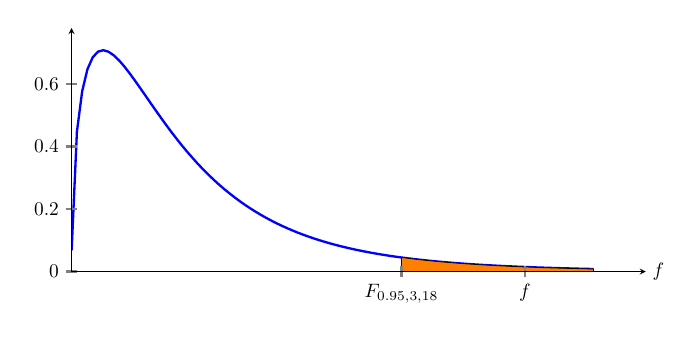
\begin{tikzpicture}[scale=.7,
				declare function={
					gamma(\z)=2.506628274631*sqrt(1/\z)+ 0.20888568*(1/\z)^(1.5)+ 0.00870357*(1/\z)^(2.5)- (174.2106599*(1/\z)^(3.5))/25920- (715.6423511*(1/\z)^(4.5))/1244160)*exp((-ln(1/\z)-1)*\z;
				},
				declare function={
					beta(\x,\y)=gamma(\x)*gamma(\y)/gamma(\x+\y);
				},
				declare function={
					fdst(\x,\a,\b) = 1 / beta(\a/2, \b/2) * (\a/\b)^(\a/2) * \x^(\a/2-1) * (1 + \a/\b*\x)^(-(\a + \b)/2);
				}
				]
				
				\begin{axis}[
					height=6cm, width=12cm,
					axis x line=center,
					xlabel=$f$,
					x label style={anchor=west},
					y label style={anchor=south},
					axis lines=left,
					xtick={3.1599, 4.343},
					xticklabels={$F_{0.95, 3, 18}$, $f$},
					axis on top,
					enlargelimits=upper,
					samples=100,
					xmin=0, ymin=0,
					domain=0.001:5, samples=100,
					legend cell align=left,
					major tick length=6,
					major tick style={very thick}
					]
					
					\addplot [very thick,blue] {fdst(x,3,18)};% \addlegendentry{$\nu_1=1,\hphantom{00} \nu_2=1$}
					\addplot [fill=orange, domain= 3.1599:5] {fdst(x,3,18)} \closedcycle;% \addlegendentry{$\nu_1=50,\hphantom{0} \nu_2=50$}
					% \addplot [very thick,purple] {fdst(x,5,2)}; \addlegendentry{$\nu_1=5,\hphantom{00} \nu_2=2$}
					
				\end{axis}
			\end{tikzpicture}    
			
			\pause
			
			Thus, $f$ lies in the critical region, and we \textbf{reject the null hypothesis} that the mean distortions from the four coatings are equal.
			
		\end{enumerate}
	\end{exampleblock}
\end{frame}


\section{MATLAB}
\begin{frame}
	\frametitle{ANOVA in MATLAB}\pause
	\begin{itemize}
		\item The computations in ANOVA are tedious and prone to human error.
		\item Usually ANOVA is conducted using software platforms such as MATLAB
	\end{itemize}
	
	\pause
	
	\begin{exampleblock}{Example 3: Investigating fuel efficiency of cars manufactured in different countries}
		The \texttt{carbig} dataset in MATLAB contains variables\footnote{For more on visualizing some of these variables, visit \url{https://www.mathworks.com/help/stats/examples/visualizing-multivariate-data.html}} for $~400$ cars from the 70s and 80s.
		The \texttt{carsmall} dataset is a subset of \texttt{carbig} (years '70, '76 and '82).\\
		
		We want to check if the true average fuel efficiency (MPG) of vehicles from
		different countries (based on the \texttt{carsmall} subset) are equal.
	\end{exampleblock}
\end{frame}

\begin{frame}
	\frametitle{ANOVA in MATLAB (cont.)}
	\begin{exampleblock}{Example 3:  Investigating fuel efficiency of cars manufactured in different countries (cont.)}
		\pause
		\begin{enumerate}[Step 1.]
			\item Examine the contents of the \texttt{example3.m} script. Run the script.\pause
			
			\item Figure 1 is a boxplot of the MPG across the different origins (6 countries).  What can you say about the variance \textit{within} each of the countries, and \textit{among} them?
			
			\includegraphics[width=.4\textwidth]{example3_boxplot}
		\end{enumerate}
	\end{exampleblock}
\end{frame}

\begin{frame}
	\frametitle{ANOVA in MATLAB (cont.)}
	\begin{exampleblock}{Example 3:  Investigating fuel efficiency of cars manufactured in different countries (cont.)}
		\pause
		\begin{enumerate}[Step 1.]\setcounter{enumi}{2}
			\item The function \texttt{anova1} generates 2 figures: the first is the ANOVA table (Figure 2)
			and the second a notched boxplot (Figure 3)
			\includegraphics[width=.5\textwidth,trim= 0 300 70 0, clip]{example3_anova}
			
			\pause
			
			\item The column \texttt{Prob>F} is the $p$-value. \pause Based on this, we \textbf{reject} the null hypothesis at any reasonable significance level.
		\end{enumerate}
	\end{exampleblock}
\end{frame}


\begin{frame}
	\frametitle{ANOVA in MATLAB (cont.)}
	\begin{exampleblock}{Example 3:  Investigating fuel efficiency of cars manufactured in different countries (cont.)}
		\pause
		\begin{enumerate}[Step 1.]\setcounter{enumi}{4}
			\item In Figure 3, we have a notched boxplot, which denotes the confidence interval of the median. What are your observations?
			
			\pause
			
			\includegraphics[width=.5\textwidth]{example3_notched}
		\end{enumerate}
	\end{exampleblock}
\end{frame}

\begin{frame}
	\frametitle{Multiple comparisons in ANOVA}\pause
	\begin{itemize}\pause
		\item If after performing a one-way ANOVA, we reject the null hypothesis, naturally we might want to find out which populations significantly differ from each
		\item Various methods have been developed for multiple pairwise comparisons (out of scope of this lecture):
		\begin{itemize}
			\item One option: perform pairwise $t$-tests between group means using the Bonferroni correction for $\alpha$ %\footnote{Refer to this week's reading on Chapter 7 for more on this}
			\item Use Tukey's range test, which performs a significance test based on the studentized range distribution
		\end{itemize}
	\end{itemize}
\end{frame}



\begin{frame}
	\frametitle{Multiple comparisons in ANOVA (cont.)}\pause
	\begin{exampleblock}{Example 3:  Investigating fuel efficiency of cars (cont.)}
		\pause
		\begin{enumerate}[Step 1.]\setcounter{enumi}{4}
			\item Uncomment lines 13 and 14 and rerun the \texttt{example3.m} script. \pause Interact with Figure 5.
			
			
			\pause
			
			\includegraphics[width=.6\textwidth]{example3_mult}
			
			\pause
			
			Which countries have significantly different average fuel efficiency?
		\end{enumerate}
	\end{exampleblock}
\end{frame}

\section{Outlook}
\begin{frame}
	\frametitle{Summary}
	\begin{itemize}
		\item The analysis of variance (ANOVA) test is used to determine whether the population means across multiple samples are equal
		\item It uses the test statistic ($f=MSG/MSE$) which is $F$-distributed
		\item Reading: Section 7.5 (Open Intro Statistics) \pause
		\item If interested, read Section 7.4 on ``power'' analysis (but we will consider this out of scope for the course)
	\end{itemize}
\end{frame}
\end{document}
%%% Local Variables:
%%% mode: latex
%%% TeX-master: t
%%% End:
